\renewcommand{\labelitemi}{$\bullet$}
\renewcommand{\labelitemii}{$\cdot$}
\renewcommand{\labelitemiii}{$\diamond$}
\renewcommand{\labelitemiv}{$\ast$}

\section{Introduction sur le métabolisme \& remise à niveau en enzymologie}

\paragraph{Objectif général de ce cours}
\begin{itemize}
    \item[$\bullet$] Comprendre le comportement général des systèmes métaboliques
    \item Aptitude à modéliser leurs dynamiques
    \item Exprimer comment les propriétés cinétiques des enzymes affecte les concentrations en métabolites et les flux
    \item Examiner comment les données expérimentales peuvent être utiliser pour identifier un modèle métabolique
    \item Interpréter ces comportements en terme de régulation biologique
    \item Généraliser au réseau de transcription des signaux
\end{itemize}

\paragraph{Pré-requis}
\begin{itemize}
    \item Connaissance sur la cinétique enzymatique
    \item Algèbre linéaire : 
    \begin{itemize}
    	\item Analyse de rang matriciel, diagonalisation, etc ...
        \item Etre familier avec les packages mathématiques comme Scilab, Maple, R ou Matlab
    \end{itemize}
    \item Système Dynamique
    \begin{itemize}
        \item Jacobienne
        \item Analyse de stabilité
    \end{itemize}
\end{itemize}

\paragraph{Outline}
\begin{enumerate}
    \item Introduction sur le métabolisme
    \item Méthode pour étudier le métabolisme
    \item Remise à niveau en cinétique enzymatique
\end{enumerate}



\subsection {Qu'est-ce que le métabolisme ?}
\begin{itemize}
    \item Usine du vivant de produits chimiques : typiquement plusieurs centaines de réactions impliquant de petites molécules 
    \item Balances
        \begin{itemize}
            \item Nutriments et produits
            \item Energie
            \item Produit du pouvroi réducteur (redox)
        \end{itemize}
    \item Turn-over rapide
    \item Les réactions chimiques souvent catalyser par des enzymes
\end{itemize} 


\begin{figure}
    \centering
    \begin{tabular}{cc}
        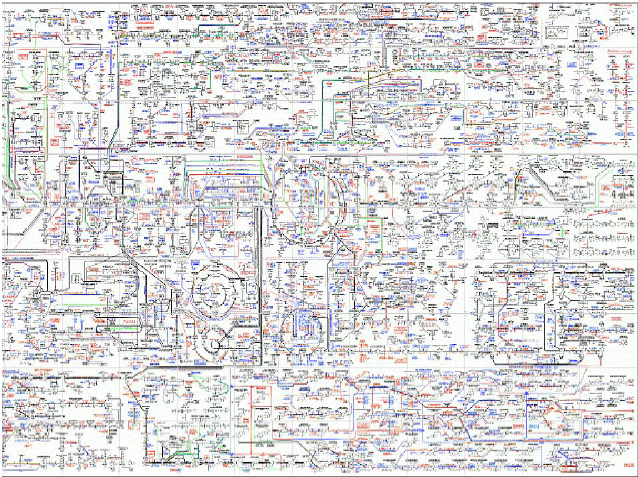
\includegraphics[width =8 cm]{Images/1.PNG} & 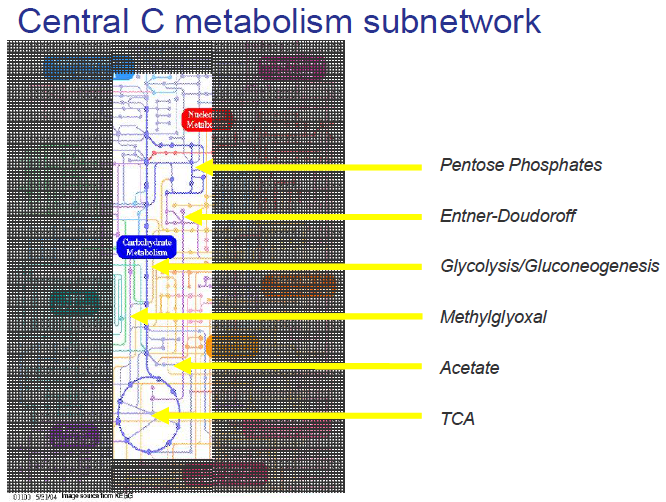
\includegraphics[width =8 cm]{Images/2.PNG} \\
        \textit{Métabolisme} & \textit{Central C metabolism subnetwork} \\
        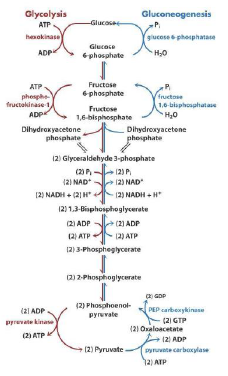
\includegraphics[width =8 cm]{Images/3.PNG} & 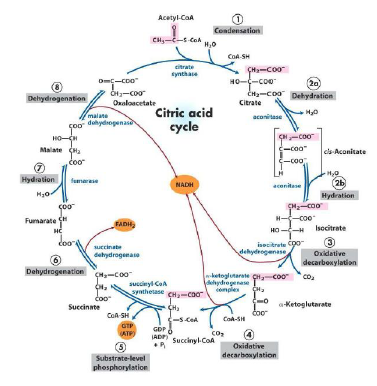
\includegraphics[width =8 cm]{Images/4.PNG} \\
        \textit{Glycolyse et néoglucogénèse}   &   \textit{TCA cycle} \\
    \end{tabular}
\end{figure}

\begin{figure}
    \centering
    \begin{tabular}{cc}
        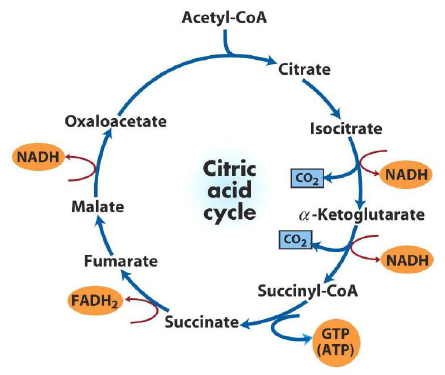
\includegraphics[width =8 cm]{Images/5.PNG}    &   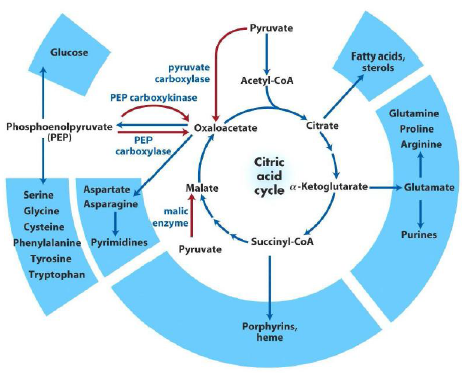
\includegraphics[width =8 cm]{Images/6.PNG} \\
        \textit{TCA cycle}     &   \textit{Anaplerosis} \\
        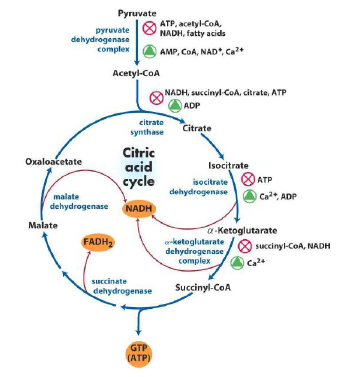
\includegraphics[width =8 cm]{Images/7.PNG}    & \\
        \textit{Régulation}    & \\
    \end{tabular}
\end{figure}


\noindent Le cycle de Krebs : gradient de protons accumulé et dissipé par une ATPases = couplage respiratoire \\

\mivbox{mivboxblue}{
cf Wikipédia \\
Réaction anaplérotique : qualifie une réaction chimique qui produit un métabolite, c'est-à-dire une espèce chimique intermédiaire d'une voie métabolique.

Anaplérose : consiste à rétablir la concentration des métabolites au sein du milieu mitochondrial afin qu'elle demeure constante et n'interrompe pas le cycle de Krebs malgré la consommation de ses métabolites par différentes biosynthèses ; élément essentiel de l'homéostasie cellulaire.

Réaction anaplérotiques majeures :
\begin{itemize}
    \item Pyruvate -(pyruvate carboxylase)-> Oxaloacétate
    \item Aspartate -(aspartate transaminase)-> Oxaloacétate
    \item Glutamate -(glutamate DH)-> $\alpha$-cétoglutarate
    \item $\beta$-oxydation des acides gras -(méthylmalonyl-CoA mutase)-> Succinyl-CoA
\end{itemize} 
}


\noindent De nombreuses enzymes sont régulées d'une manière allostériques, effecteur en lien avec la charge. 


\subsection{Méthodes pour étudier le métabolisme}

\begin{itemize}
    \item Métabolomique : identification et quantification des métabolites 
    \item Fluxomics : inférence ou prédiction du taux de réactions métaboliques dans les systèmes biologiques (cf Wikipedia)
    \item Outils analytiques basés sur :
        \begin{itemize}
            \item Résonance magnétique nucléaire (NMR)
            \item Spectrométrie de masse (MS)
            \item Chromatographie liquide (LC)
        \end{itemize}
\end{itemize}

\noindent Méthode de flux métabolique : vitesse réactionnelle lorsqu'il opère à l'état stationnaire

\begin{figure}[!h]
    \centering
    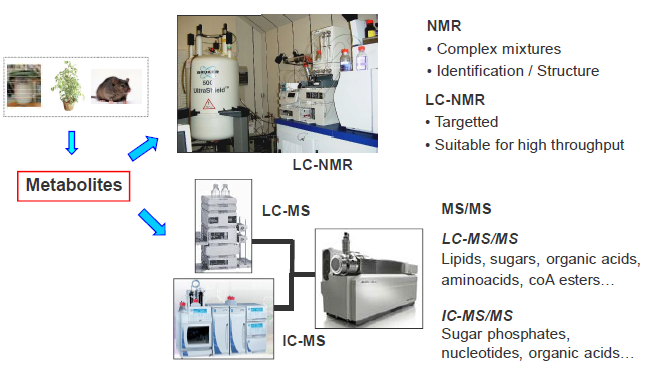
\includegraphics{Images/8.PNG}
    \caption{Métabolomique}
\end{figure}

\noindent La résonance magnétique nucléaire (NMR) permet une analyse structurale. C'est une méthode peu sensible : molarité > mm , il ne détecte que les métabolites présents en grande quantités.  

\noindent MS/MS : sépare selon la masse et permet d'identifier les produits de fragmentation.

\begin{figure}
    \centering
    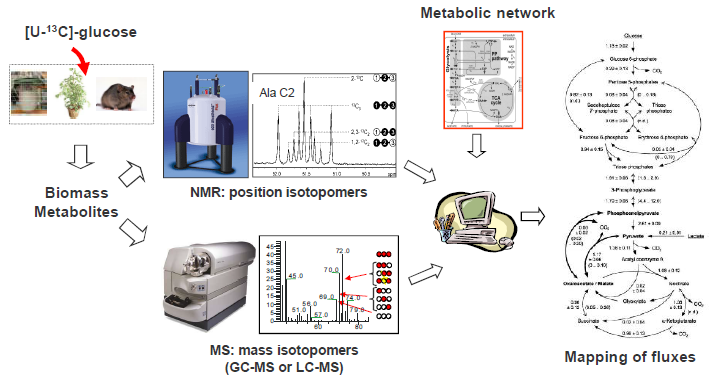
\includegraphics{Images/9.PNG}
    \caption{Flux measurements}
\end{figure}


\paragraph{}Il est plus difficile de chercher à mesurer les flux internes. La méthode de marquage des molécules ($^{13}C$, $^{15}N$) peut être utilisée. $\Rightarrow$ mesure la distribution des isotopomères des métabolites = distribution d'un marquage $\Rightarrow$ modèle

\paragraph{} Exemple :

Glucose marqué $\Rightarrow$ acide aminé marqué $\Rightarrow$ voie de biosynthèse connus

$\hookrightarrow$ modèle $\Rightarrow$ à partir de la distribution des isotopomères on peut représenter les flux

\mivbox{mivboxblue}{Isotopomères : }


\begin{figure}[!ht]
    \centering
    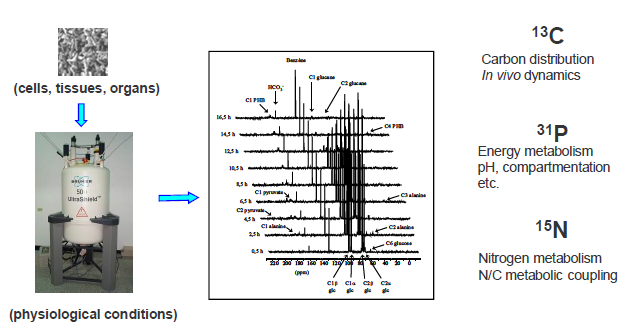
\includegraphics{Images/10.PNG}
    \caption{\textit{in vivo} NMR}
\end{figure}

\paragraph{}NMR peut être utilisé \textit{in vivo} uniquement si la molécule est majoritairement détectée.
$^3P$ : très utilme pour mesurer la charge énergétique, le pH


\subsection{Cinétique enzymatique : Michaelis-Menten}

Une \textbf{enzyme} est une protéine catalysant une réaction, elle facilite la réaction avec aucun changement de conformation.

$$E + S  \leftrightarrows ES \rightarrow E + P$$

\paragraph{}Action cinétique de la masse (Mass action kinetics) :
\begin{align*}
v_1 &=k_1E.S - k_{-1}ES\\
v_2 &=k_2ES
\end{align*}

\paragraph{}Quasi steady-state :
$$v_1=v_2=v$$
$$E + ES = E_0$$

\begin{align*}
&v = E_0 \frac{k_ES}{1+ \frac{S}{K_m}} \text{ taux de réaction } (M.s^{-1}) \\
&K_m = \frac{k_{-1}+k_{cat}}{k_1} \text{ Constance de Michaelis } (M)\\
&k_E =\frac{k_{cat}}{K_m} \text{ efficience catalytique } (M^{-1}.s^{-1})\\
&k_{cat} \text{ est le taux de turn-over maximal } (s^{-1})
\end{align*}

\paragraph{Michaelis-Menten Réversible}

$$E + S \leftrightarrows ES \leftrightarrows E + P$$

\begin{center}\fbox{$v=E_0 \frac{k_+S - k_-P}{1+ \frac{1}{K_S} + \frac{P}{K_P}}$}\end{center}
\noindent Il s'agit de l'\textcolor{red}{expression par défaut} pour la modélisation cinétique, équivalent quand $k_{-}=0$, parce qu'il explique le phénomène de competitive product inhibition.


\paragraph{Inhibition compétitive}
\begin{align*}
    E & + S 	\leftrightarrows ES \leftrightarrows & E + P \\
    \Updownarrow &  &  \Updownarrow \\
    E.I &  & E.I
\end{align*}



$$v = E_0 \frac{k_+S- k_-P}{1 + \frac{1}{K_S} + \frac{P}{K_P} + \frac{I}{K_{Ic}}}$$


\paragraph{Autres inhibitions}
\paragraph{}\noindent Non-compétitive (plus efficace à forte concentration en substrat)
$$v=E_0 \frac{k_+S-k_-P}{1+(\frac{S}{K_S}+\frac{P}{K_P})(1+\frac{I}{K_{Iu}})}$$


\noindent Mixed
$v=E_0 \frac{k_+S-k_-P}{1+(\frac{S}{K_S}+\frac{P}{K_P})(1+\frac{I}{K_{Iu}})+\frac{I}{K_{Ic}}}$




\paragraph{Multiples substrats et produits}
Si les substrats et les produits se lient indépendamment et dans un ordre aléatoire :

$$v=E_0\frac{k^+_{cat} \prod_{i} \frac{S_i}{K_{S_i}}-k^-_{cat} \prod_{j} \frac{P_j}{K_{P_j}}}{\prod_{i} (1+ \frac{S_i}{K_{S_i}}) + \prod_{j}(1+\frac{P_j}{K_{P_j}})-1}$$


\noindent source : 'Convenience kinetics' Liebermeister \& Klipp, 2006, Theoret. Biol. Med. Mod. 3:41




\paragraph{Relation de Haldane}
La contrainte de l'équilibre : $$K_{eq}=\frac{k^+_{cat} \prod_{j}K_{P_j}}{k^-_{cat} \prod_{i}K_{S_i}}$$


\paragraph{Cinétique enzymatique \& Thermodynamique}
Si on appelle $\Gamma$ le rapport de l'action de masse (mass action ratio) : $$ \Gamma = \frac{\prod_{j}P_j}{\prod_{i}S_i} = K_{eq}exp(\Delta G'/RT)$$

\noindent La cinétique enzymatique peut être divisée en 3 termes : $$v=k^+_{cat}E_0.f(S_i,P_j).(1-\Gamma/K_{eq})$$
\begin{itemize}
\item $1^{er}$ terme : $k^+_{cat}E_0$ correspond à la capacité enzymatique
\item $2^{nd}$ terme : $0 < f(S_i,P_j) < 1$ est le terme de saturation enzymatique. 
\textit{Comme un exercice, écrire ce terme pour la cinétique de Michaelis-Menten réversible}.
\item $3^{ème}$ terme : terme purement thermodynamique, il est indépendant des propriétés enzymatiques $\frac{1-\Gamma}{K_{eq}}=1-exp (\Delta G'/RT)$
\end{itemize}



\textbf{Cooperativity ?}
Equation de Hill : $$v=E_0 \frac{k_{cat}(S/K_{0.5})^h}{1+(S/K_{0.5})^h}$$

\noindent $h$ est le coefficient de Hill. Typiquement : $0.5<h<4$.
Cette équation est purement empirique (actuellement érronné pour $S<<K_{0.5}$).
$K_{0.5}$ est une constante phénoménologique (pas un $K_m$ !).

\paragraph{2-site cooperative binding}
Equation d'Adair :
$$v=2E_0k_{cat} \frac{S/K_1 + S^2 / K_1K_2}{1+2S/K_1+S^2/K_1K_2}$$
\noindent reastically captures site dependencies.

\paragraph{Saturation}
$E+S \leftrightarrows ES$
$E+ES=E_0$
$\frac{E.S}{ES}=\frac{k_{-1}}{k_1}=k_d$
$Y=\frac{ES}{E_0}=\frac{S/K_d}{1+S/K_d}$


\paragraph{Pour aller plus loin ...}
\begin{itemize}
\item \textit{Understanding the Control of Metabolism}, by David Fell, Portland Press, London, 1997
\item \textit{Fundamentals of Enzyme Kinetics}, by Athel Cornish-Bowden, Portland Press, London, 2004
\end{itemize}


\paragraph{Pour les TP :}
\begin{itemize}
\item The practical course will rely heavily on the theoretical course
\item Familiarize yourself with the COPASI modeling environment
http://www.copasi.org  (COPASI handbook)
\item  Refresh your course in linear algebra
\item Be prepared to use your favourite mathematical package
such as Octave, Scilab, Maple, R or Matlab
\item You will be evaluated on the practical course
\end{itemize}
